\documentclass[11pt]{article}
\usepackage[utf8]{inputenc}
\usepackage[T1]{fontenc}
\usepackage[spanish]{babel}
\usepackage[margin=2.3cm]{geometry}
\usepackage{amsmath}
\usepackage{graphicx}
\usepackage{xcolor}
\usepackage[colorlinks=true,urlcolor=blue!60!black,linkcolor=black]{hyperref}
\usepackage{parskip}

\title{\textbf{Imágenes candidatas de la bibliografía}\\[2pt]
\large Propuestas de figuras para la monografía --- para revisión}
\author{}\date{}

\begin{document}
\maketitle
\vspace{-2.2em}

\noindent\textbf{Cómo leer este documento.} Las figuras de \emph{resultados} de otros
papers tienen \emph{copyright}: copiarlas exige permiso del editor. Lo limpio y rápido es
\textbf{redibujarlas como esquema propio} (como ya hicimos con las 6 figuras nuevas) y
poner en el pie ``\emph{Esquema propio, basado en} \texttt{[ref]}''. Abajo, en la
\textbf{Parte A}, ves \emph{los esquemas que yo dibujaría} (ya hechos, listos para insertar);
en la \textbf{Parte B}, los papers que conviene \emph{citar} para comparar (sin copiar imagen).

\hrulefill

\section*{Parte A --- Esquemas propios propuestos (ya dibujados)}

\subsection*{A1. Lámina de corriente y modo \emph{tearing} (islas / plasmoides)\quad\textcolor{red}{\textbf{[alta prioridad]}}}
\begin{center}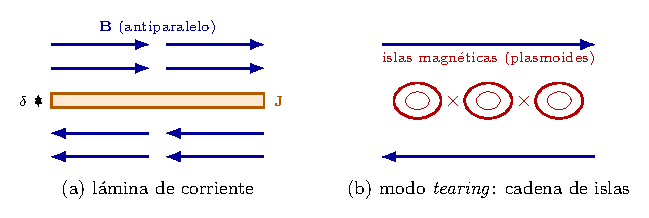
\includegraphics[width=0.96\textwidth]{figuras/tikz_src/corriente_tearing.pdf}\end{center}
\textbf{Dónde:} Cap.~6, sección de leyes de potencia. \textbf{Por qué:} la revisión señaló que el
exponente $\Omega^{\max}\!\propto\!\sigma^{1.22}$ y el \emph{tearing} ``se afirman pero no se muestran''.
Este esquema los ilustra. \textbf{Basado en:} Furth, Killeen \& Rosenbluth (1963)
[\href{https://doi.org/10.1063/1.1706761}{doi}]; Lyubarsky (2005)
[\href{https://arxiv.org/abs/astro-ph/0501392}{arXiv}].

\subsection*{A2. Reconexión de Sweet--Parker ($\delta\propto S^{-1/2}$)\quad\textcolor{red}{\textbf{[alta prioridad]}}}
\begin{center}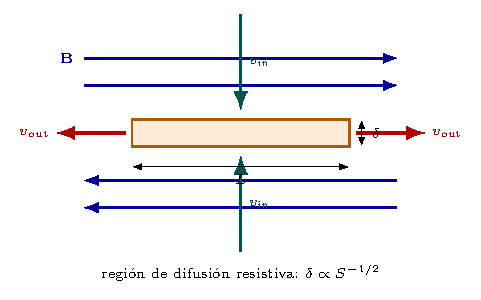
\includegraphics[width=0.72\textwidth]{figuras/tikz_src/sweet_parker.pdf}\end{center}
\textbf{Dónde:} Cap.~6 (leyes de potencia) o Cap.~3. \textbf{Por qué:} sustenta el ``piso''
$\delta\propto\sigma^{-1/2}$ que usamos como referencia del exponente. \textbf{Basado en:}
Parker (1957) [\href{https://doi.org/10.1029/JZ062i004p00509}{doi}].

\subsection*{A3. Estabilización por tensión magnética ($\gamma$ vs.\ $\mathbf k\cdot\mathbf B$)}
\begin{center}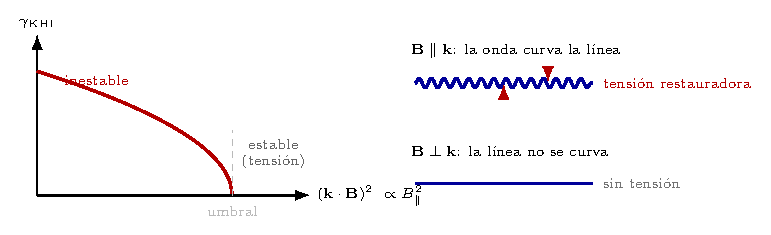
\includegraphics[width=0.98\textwidth]{figuras/tikz_src/tension_estabilizacion.pdf}\end{center}
\textbf{Dónde:} Cap.~3 (MHD ideal) o Cap.~6 (campañas B/C). \textbf{Por qué:} explica por qué
$B_y$ ($\parallel\mathbf k$) estabiliza vía tensión y $B_x$ ($\perp\mathbf k$) no. \textbf{Basado en:}
Osmanov et al.\ (2008) [\href{https://doi.org/10.1051/0004-6361:200809605}{doi}];
Chow et al.\ (2023) [\href{https://arxiv.org/abs/2305.00036}{arXiv}]; Bodo et al.\ (2004).

\hrulefill

\section*{Parte B --- Para comparar / citar (no copiar imagen)}
\begin{itemize}
\item \textbf{Mizuno et al.\ (2013)} --- \emph{nuestro setup base}; snapshots de la KHI resistiva.
  \href{https://doi.org/10.1088/0067-0049/205/1/7}{doi} \quad(\texttt{mizuno-2013})
\item \textbf{Gomes et al.\ (2017)} --- KHI ideal vs.\ resistiva 2D, muy alineado con nuestro caso.
  \href{https://doi.org/10.5540/tema.2017.018.02.0317}{doi} \quad(\texttt{gomes-2017})
\item \textbf{Palenzuela et al.\ (2009)} --- RRMHD, KHI y reconexión.
  \href{https://doi.org/10.1111/j.1365-2966.2009.14454.x}{doi} \quad(\texttt{palenzuela-2009})
\item \textbf{Lecoanet et al.\ (2016)} --- benchmark KHI (resistividad necesaria / bien planteado).
  \href{https://doi.org/10.1093/mnras/stv2564}{doi} \quad(\texttt{lecoanet2016})
\item \textbf{Bucciantini \& Del Zanna (2006)} --- KHI en nebulosas de viento de púlsar.
  \href{https://doi.org/10.1051/0004-6361:20054491}{doi} \quad(\texttt{bucciantini-2006})
\end{itemize}

\hrulefill

\section*{Cómo citarlas}
\textbf{Opción 1 --- redibujar (recomendado).} Sin permiso. Pie: ``\emph{Esquema propio, basado en}
\texttt{\textbackslash parencite\{furth1963\}}'' o ``\emph{Adaptado de}~\dots''. Es lo de la Parte~A.

\textbf{Opción 2 --- copiar la figura del paper.} Copyright del editor (AAS, OUP/MNRAS, A\&A, AIP\dots).
Requiere \emph{permiso} (RightsLink; algunos arXiv/AAS son CC-BY) y \emph{atribución}:
``\emph{Figura tomada de} \texttt{\textbackslash textcite\{mizuno-2013\}}. © AAS, reproducida con permiso.''

\medskip
\noindent\textbf{Recomendación:} usar Opción~1 para la Parte~A; para la Parte~B, citar en el texto sin copiar.
\end{document}
